% Options for packages loaded elsewhere
\PassOptionsToPackage{unicode}{hyperref}
\PassOptionsToPackage{hyphens}{url}
%
\documentclass[
]{article}
\usepackage{amsmath,amssymb}
\usepackage{lmodern}
\usepackage{iftex}
\ifPDFTeX
  \usepackage[T1]{fontenc}
  \usepackage[utf8]{inputenc}
  \usepackage{textcomp} % provide euro and other symbols
\else % if luatex or xetex
  \usepackage{unicode-math}
  \defaultfontfeatures{Scale=MatchLowercase}
  \defaultfontfeatures[\rmfamily]{Ligatures=TeX,Scale=1}
\fi
% Use upquote if available, for straight quotes in verbatim environments
\IfFileExists{upquote.sty}{\usepackage{upquote}}{}
\IfFileExists{microtype.sty}{% use microtype if available
  \usepackage[]{microtype}
  \UseMicrotypeSet[protrusion]{basicmath} % disable protrusion for tt fonts
}{}
\makeatletter
\@ifundefined{KOMAClassName}{% if non-KOMA class
  \IfFileExists{parskip.sty}{%
    \usepackage{parskip}
  }{% else
    \setlength{\parindent}{0pt}
    \setlength{\parskip}{6pt plus 2pt minus 1pt}}
}{% if KOMA class
  \KOMAoptions{parskip=half}}
\makeatother
\usepackage{xcolor}
\IfFileExists{xurl.sty}{\usepackage{xurl}}{} % add URL line breaks if available
\IfFileExists{bookmark.sty}{\usepackage{bookmark}}{\usepackage{hyperref}}
\hypersetup{
  pdftitle={Homework 5: Propensity Score Analysis --- Stratification and Regression},
  pdfauthor={Xuange Liang},
  hidelinks,
  pdfcreator={LaTeX via pandoc}}
\urlstyle{same} % disable monospaced font for URLs
\usepackage{longtable,booktabs,array}
\usepackage{calc} % for calculating minipage widths
% Correct order of tables after \paragraph or \subparagraph
\usepackage{etoolbox}
\makeatletter
\patchcmd\longtable{\par}{\if@noskipsec\mbox{}\fi\par}{}{}
\makeatother
% Allow footnotes in longtable head/foot
\IfFileExists{footnotehyper.sty}{\usepackage{footnotehyper}}{\usepackage{footnote}}
\makesavenoteenv{longtable}
\usepackage{graphicx}
\makeatletter
\def\maxwidth{\ifdim\Gin@nat@width>\linewidth\linewidth\else\Gin@nat@width\fi}
\def\maxheight{\ifdim\Gin@nat@height>\textheight\textheight\else\Gin@nat@height\fi}
\makeatother
% Scale images if necessary, so that they will not overflow the page
% margins by default, and it is still possible to overwrite the defaults
% using explicit options in \includegraphics[width, height, ...]{}
\setkeys{Gin}{width=\maxwidth,height=\maxheight,keepaspectratio}
% Set default figure placement to htbp
\makeatletter
\def\fps@figure{htbp}
\makeatother
\setlength{\emergencystretch}{3em} % prevent overfull lines
\providecommand{\tightlist}{%
  \setlength{\itemsep}{0pt}\setlength{\parskip}{0pt}}
\setcounter{secnumdepth}{5}
% Shared LaTeX style for homework submissions
\usepackage{microtype}
\usepackage{booktabs}
\usepackage{longtable}
\usepackage{array}
\usepackage{caption}
\usepackage{fancyhdr}
\usepackage{titlesec}
\usepackage{setspace}
\usepackage{float}
\usepackage{graphicx}
\usepackage[table]{xcolor}
\usepackage{enumitem}
\usepackage[most]{tcolorbox}
\usepackage{geometry}

\geometry{left=2.2cm, right=2.2cm, top=2.5cm, bottom=2.5cm}

\definecolor{TitleBlue}{HTML}{0B3C5D}
\definecolor{SoftGray}{HTML}{F6F8FA}

\setstretch{1.15}
\setlength{\parskip}{4pt}
\setlength{\parindent}{0pt}

\AtBeginEnvironment{longtable}{\small}

\titleformat{\section}{\large\bfseries\color{TitleBlue}}{\thesection}{0.6em}{}
\titleformat{\subsection}{\normalsize\bfseries\color{TitleBlue}}{\thesubsection}{0.6em}{}

\captionsetup{
  font=small,
  labelfont=bf
}

\rowcolors{2}{SoftGray}{white}
\setlist[itemize]{leftmargin=*, topsep=2pt, itemsep=1pt}
\setlist[enumerate]{leftmargin=*, topsep=2pt, itemsep=1pt}

\pagestyle{fancy}
\fancyhf{}
\fancyhead[L]{\small\nouppercase{\leftmark}}
\fancyhead[R]{\small P8586 Applied Methods}
\fancyfoot[C]{\thepage}
\setlength{\headheight}{15pt}
\addtolength{\topmargin}{-1pt}
\renewcommand{\headrulewidth}{0.4pt}

\AtBeginDocument{
  \hypersetup{
    colorlinks=true,
    linkcolor=TitleBlue,
    urlcolor=TitleBlue,
    citecolor=TitleBlue
  }
}

\AtBeginDocument{
  \let\oldtableofcontents\tableofcontents
  \renewcommand{\tableofcontents}{%
    \oldtableofcontents
    \clearpage
  }
}

\ifLuaTeX
  \usepackage{selnolig}  % disable illegal ligatures
\fi

\title{Homework 5: Propensity Score Analysis --- Stratification and
Regression}
\author{Xuange Liang}
\date{March 31, 2026}

\begin{document}
\maketitle

{
\setcounter{tocdepth}{3}
\tableofcontents
}
\hypertarget{introduction}{%
\section{Introduction}\label{introduction}}

In this homework, I used \textbf{propensity score (PS) stratification}
and \textbf{PS regression} to study the association between
intraventricular hemorrhage (IVH) and neonatal mortality among very low
birth weight (VLBW) infants. The cohort includes 514 infants with birth
weight below 1,600 g born at Duke University Medical Center from 1981 to
1987. The exposure is IVH (\texttt{ivh2\ =\ 1} in 84 infants, 16.3\%),
and the outcome is in-hospital death (\texttt{dead\ =\ 1} in 99 infants,
19.3\%).

This homework extends the earlier analyses from HW1, HW3, and HW4.
Instead of adjusting for confounders only through conventional
regression, I first estimated each infant's probability of having IVH
based on measured baseline characteristics, then used that propensity
score in two additional ways:

\begin{itemize}
\tightlist
\item
  \textbf{PS stratification:} divide the cohort into five quintile
  strata and compare outcomes across exposure groups within strata.
\item
  \textbf{PS regression:} include the estimated PS directly in the
  outcome model as an adjustment variable.
\end{itemize}

I also compared the HW5 results with the unadjusted model from HW1, the
multivariable model from HW1, the PS-matched results from HW3, and the
PS-IPTW results from HW4.

\begin{center}\rule{0.5\linewidth}{0.5pt}\end{center}

\hypertarget{requirement-1-ps-step-1-model}{%
\section{Requirement 1: PS Step 1
Model}\label{requirement-1-ps-step-1-model}}

\hypertarget{propensity-score-model-specification}{%
\subsection{Propensity Score Model
Specification}\label{propensity-score-model-specification}}

Following the homework instructions, I fit a \textbf{simple PS step 1
logistic regression model without interaction terms}, using IVH as the
response variable and the measured baseline confounders as predictors:

\begin{itemize}
\tightlist
\item
  Pneumothorax (\texttt{pneumo})
\item
  Multiple gestation (\texttt{twin})
\item
  Mode of delivery (\texttt{delivery\_new})
\item
  Birth location (\texttt{inout\_new})
\item
  Birth weight category (\texttt{bwt\_cat})
\item
  Gestational age category (\texttt{gest\_cat})
\end{itemize}

\hypertarget{roc-curve-and-model-fit}{%
\subsection{ROC Curve and Model Fit}\label{roc-curve-and-model-fit}}

\begin{figure}
\centering
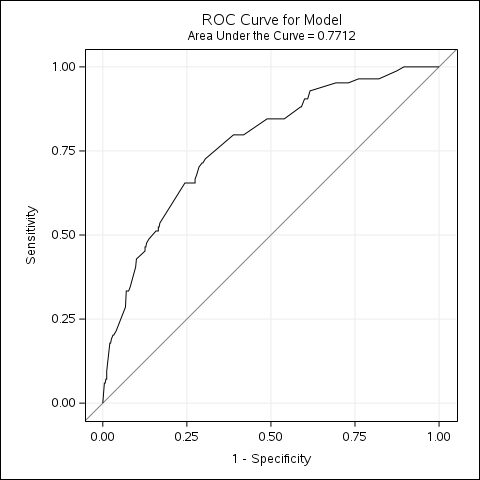
\includegraphics[width=0.6\textwidth,height=\textheight]{fig_roc_ps_model.png}
\caption{ROC Curve for PS Step 1 Model}
\end{figure}

The main-effects PS model had \textbf{C-statistic = 0.771}, indicating
acceptable discrimination between infants with and without IVH. This is
the same step 1 model used in HW3 and HW4, which supports consistency
across the propensity score analyses.

\hypertarget{model-a-parameter-estimates}{%
\subsection{Model A: Parameter
Estimates}\label{model-a-parameter-estimates}}

\begin{longtable}[]{@{}llccc@{}}
\toprule
Covariate & Level & OR & 95\% CI & p-value \\
\midrule
\endhead
Pneumothorax & Yes vs.~No & 3.712 & (2.073, 6.648) & \textless{}
0.001 \\
Multiple Gestation & Yes vs.~No & 0.319 & (0.136, 0.751) & 0.009 \\
Mode of Delivery & Vaginal vs.~C-Section & 2.178 & (1.234, 3.844) &
0.007 \\
Birth Location & Transport vs.~Duke & 2.571 & (1.458, 4.535) & 0.001 \\
Birth Weight & \textless{} 1000g vs.~\(\geq\) 1300g & 1.954 & (0.785,
4.861) & 0.150 \\
Birth Weight & 1000-1299g vs.~\(\geq\) 1300g & 1.564 & (0.711, 3.440) &
0.266 \\
Gestational Age & \textless{} 28 wks vs.~\(\geq\) 32 wks & 5.093 &
(1.028, 25.221) & 0.046 \\
Gestational Age & 28-31 wks vs.~\(\geq\) 32 wks & 5.063 & (1.145,
22.400) & 0.033 \\
\bottomrule
\end{longtable}

\emph{C-statistic = 0.771. Significant predictors of IVH were
pneumothorax, multiple gestation, mode of delivery, birth location, and
gestational age.}

\hypertarget{ps-quintile-definition}{%
\subsection{PS Quintile Definition}\label{ps-quintile-definition}}

After estimating the PS for each infant, I ranked the predicted scores
and created \textbf{five PS quintile strata}. All 514 infants were
retained.

\begin{longtable}[]{@{}rlrrr@{}}
\toprule
Stratum & PS Range & Total N & No IVH & IVH \\
\midrule
\endhead
1 & 0.0036-0.0380 & 103 & 100 & 3 \\
2 & 0.0400-0.0999 & 103 & 96 & 7 \\
3 & 0.0999-0.1621 & 102 & 95 & 7 \\
4 & 0.1621-0.2479 & 103 & 79 & 24 \\
5 & 0.2479-0.6988 & 103 & 60 & 43 \\
\bottomrule
\end{longtable}

This table shows that infants with IVH were concentrated in the
higher-propensity strata. More than half of the exposed infants were in
stratum 5, whereas only 3 infants with IVH were in stratum 1.

\begin{center}\rule{0.5\linewidth}{0.5pt}\end{center}

\hypertarget{requirement-2-table-1-baseline-characteristics-within-ps-strata}{%
\section{Requirement 2: Table 1 --- Baseline Characteristics Within PS
Strata}\label{requirement-2-table-1-baseline-characteristics-within-ps-strata}}

The homework asked for Table 1 to be presented by strata, with
\textbf{column percentages by exposure group}. Because the first three
strata contained very few IVH-exposed infants, I report descriptive
percentages without emphasizing formal p-values. The main purpose of
this table is to show how the exposed and unexposed infants compare
within each PS risk band.

\hypertarget{table-1-baseline-characteristics-by-ivh-status-within-ps-quintile-strata}{%
\subsection{Table 1: Baseline Characteristics by IVH Status Within PS
Quintile
Strata}\label{table-1-baseline-characteristics-by-ivh-status-within-ps-quintile-strata}}

\begin{longtable}[]{@{}llcc@{}}
\toprule
Stratum & Covariate & No IVH & IVH \\
\midrule
\endhead
\textbf{1} & \textbf{PS range 0.0036-0.0380; N = 103} & \textbf{100} &
\textbf{3} \\
& Pneumothorax: No & 100 (100.0\%) & 3 (100.0\%) \\
& Pneumothorax: Yes & 0 (0.0\%) & 0 (0.0\%) \\
& Multiple gestation: Singleton & 38 (38.0\%) & 1 (33.3\%) \\
& Multiple gestation: Multiple & 62 (62.0\%) & 2 (66.7\%) \\
& Delivery: C-Section & 73 (73.0\%) & 2 (66.7\%) \\
& Delivery: Vaginal & 27 (27.0\%) & 1 (33.3\%) \\
& Birth location: Born at Duke & 95 (95.0\%) & 3 (100.0\%) \\
& Birth location: Transport & 5 (5.0\%) & 0 (0.0\%) \\
& Birth weight: \textless1000 g & 9 (9.0\%) & 0 (0.0\%) \\
& Birth weight: 1000-1299 g & 45 (45.0\%) & 2 (66.7\%) \\
& Birth weight: 1300-1599 g & 46 (46.0\%) & 1 (33.3\%) \\
& Gestational age: \textless28 weeks & 3 (3.0\%) & 0 (0.0\%) \\
& Gestational age: 28-31 weeks & 48 (48.0\%) & 2 (66.7\%) \\
& Gestational age: \$\geq\$32 weeks & 49 (49.0\%) & 1 (33.3\%) \\
\textbf{2} & \textbf{PS range 0.0400-0.0999; N = 103} & \textbf{96} &
\textbf{7} \\
& Pneumothorax: No & 84 (87.5\%) & 5 (71.4\%) \\
& Pneumothorax: Yes & 12 (12.5\%) & 2 (28.6\%) \\
& Multiple gestation: Singleton & 77 (80.2\%) & 5 (71.4\%) \\
& Multiple gestation: Multiple & 19 (19.8\%) & 2 (28.6\%) \\
& Delivery: C-Section & 81 (84.4\%) & 7 (100.0\%) \\
& Delivery: Vaginal & 15 (15.6\%) & 0 (0.0\%) \\
& Birth location: Born at Duke & 88 (91.7\%) & 7 (100.0\%) \\
& Birth location: Transport & 8 (8.3\%) & 0 (0.0\%) \\
& Birth weight: \textless1000 g & 26 (27.1\%) & 0 (0.0\%) \\
& Birth weight: 1000-1299 g & 49 (51.0\%) & 6 (85.7\%) \\
& Birth weight: 1300-1599 g & 21 (21.9\%) & 1 (14.3\%) \\
& Gestational age: \textless28 weeks & 9 (9.4\%) & 2 (28.6\%) \\
& Gestational age: 28-31 weeks & 77 (80.2\%) & 5 (71.4\%) \\
& Gestational age: \$\geq\$32 weeks & 10 (10.4\%) & 0 (0.0\%) \\
\textbf{3} & \textbf{PS range 0.0999-0.1621; N = 102} & \textbf{95} &
\textbf{7} \\
& Pneumothorax: No & 86 (90.5\%) & 7 (100.0\%) \\
& Pneumothorax: Yes & 9 (9.5\%) & 0 (0.0\%) \\
& Multiple gestation: Singleton & 85 (89.5\%) & 7 (100.0\%) \\
& Multiple gestation: Multiple & 10 (10.5\%) & 0 (0.0\%) \\
& Delivery: C-Section & 30 (31.6\%) & 3 (42.9\%) \\
& Delivery: Vaginal & 65 (68.4\%) & 4 (57.1\%) \\
& Birth location: Born at Duke & 89 (93.7\%) & 7 (100.0\%) \\
& Birth location: Transport & 6 (6.3\%) & 0 (0.0\%) \\
& Birth weight: \textless1000 g & 27 (28.4\%) & 3 (42.9\%) \\
& Birth weight: 1000-1299 g & 32 (33.7\%) & 0 (0.0\%) \\
& Birth weight: 1300-1599 g & 36 (37.9\%) & 4 (57.1\%) \\
& Gestational age: \textless28 weeks & 24 (25.3\%) & 0 (0.0\%) \\
& Gestational age: 28-31 weeks & 69 (72.6\%) & 7 (100.0\%) \\
& Gestational age: \$\geq\$32 weeks & 2 (2.1\%) & 0 (0.0\%) \\
\textbf{4} & \textbf{PS range 0.1621-0.2479; N = 103} & \textbf{79} &
\textbf{24} \\
& Pneumothorax: No & 67 (84.8\%) & 20 (83.3\%) \\
& Pneumothorax: Yes & 12 (15.2\%) & 4 (16.7\%) \\
& Multiple gestation: Singleton & 73 (92.4\%) & 22 (91.7\%) \\
& Multiple gestation: Multiple & 6 (7.6\%) & 2 (8.3\%) \\
& Delivery: C-Section & 14 (17.7\%) & 4 (16.7\%) \\
& Delivery: Vaginal & 65 (82.3\%) & 20 (83.3\%) \\
& Birth location: Born at Duke & 68 (86.1\%) & 20 (83.3\%) \\
& Birth location: Transport & 11 (13.9\%) & 4 (16.7\%) \\
& Birth weight: \textless1000 g & 52 (65.8\%) & 13 (54.2\%) \\
& Birth weight: 1000-1299 g & 21 (26.6\%) & 8 (33.3\%) \\
& Birth weight: 1300-1599 g & 6 (7.6\%) & 3 (12.5\%) \\
& Gestational age: \textless28 weeks & 39 (49.4\%) & 13 (54.2\%) \\
& Gestational age: 28-31 weeks & 40 (50.6\%) & 10 (41.7\%) \\
& Gestational age: \$\geq\$32 weeks & 0 (0.0\%) & 1 (4.2\%) \\
\textbf{5} & \textbf{PS range 0.2479-0.6988; N = 103} & \textbf{60} &
\textbf{43} \\
& Pneumothorax: No & 20 (33.3\%) & 15 (34.9\%) \\
& Pneumothorax: Yes & 40 (66.7\%) & 28 (65.1\%) \\
& Multiple gestation: Singleton & 57 (95.0\%) & 42 (97.7\%) \\
& Multiple gestation: Multiple & 3 (5.0\%) & 1 (2.3\%) \\
& Delivery: C-Section & 23 (38.3\%) & 11 (25.6\%) \\
& Delivery: Vaginal & 37 (61.7\%) & 32 (74.4\%) \\
& Birth location: Born at Duke & 26 (43.3\%) & 17 (39.5\%) \\
& Birth location: Transport & 34 (56.7\%) & 26 (60.5\%) \\
& Birth weight: \textless1000 g & 32 (53.3\%) & 27 (62.8\%) \\
& Birth weight: 1000-1299 g & 23 (38.3\%) & 14 (32.6\%) \\
& Birth weight: 1300-1599 g & 5 (8.3\%) & 2 (4.7\%) \\
& Gestational age: \textless28 weeks & 39 (65.0\%) & 25 (58.1\%) \\
& Gestational age: 28-31 weeks & 21 (35.0\%) & 18 (41.9\%) \\
& Gestational age: \$\geq\$32 weeks & 0 (0.0\%) & 0 (0.0\%) \\
\bottomrule
\end{longtable}

\textbf{Plain-language interpretation of Table 1:}

The stratified table shows that the infants in higher PS strata were
much sicker and more premature overall. By stratum 5, both the IVH and
No-IVH groups had high frequencies of pneumothorax, lower birth weight,
and gestational age below 28 weeks. In contrast, stratum 1 mainly
contained larger and less premature infants.

Within each stratum, the exposed and unexposed infants looked more
similar than they did in the original cohort. That is the main purpose
of PS stratification. However, overlap was still limited in the low-PS
region because there were only 3 IVH infants in stratum 1 and 7 IVH
infants in each of strata 2 and 3. So the stratified comparison is
improved, but not perfect.

\begin{center}\rule{0.5\linewidth}{0.5pt}\end{center}

\hypertarget{requirement-3-distribution-of-patients-and-propensity-scores-across-strata}{%
\section{Requirement 3: Distribution of Patients and Propensity Scores
Across
Strata}\label{requirement-3-distribution-of-patients-and-propensity-scores-across-strata}}

\hypertarget{figure-1-proportion-of-patients-at-each-stratum-by-exposure-group}{%
\subsection{Figure 1: Proportion of Patients at Each Stratum by Exposure
Group}\label{figure-1-proportion-of-patients-at-each-stratum-by-exposure-group}}

\begin{figure}
\centering
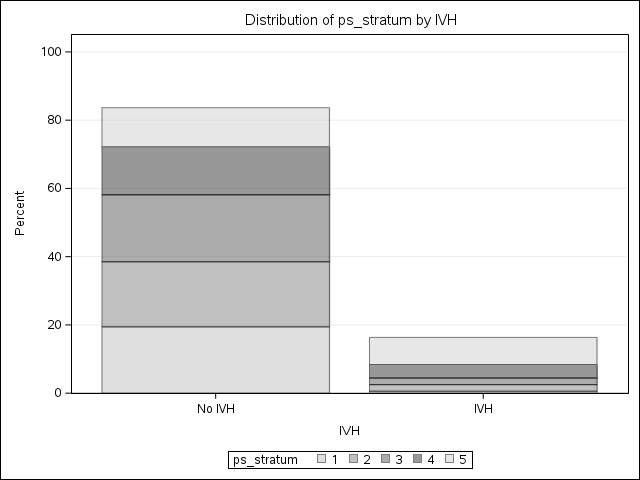
\includegraphics[width=0.8\textwidth,height=\textheight]{fig_stratum_proportion_sas.png}
\caption{Proportion of patients at each stratum by exposure group}
\end{figure}

Figure 1 shows that the IVH group was concentrated in the upper PS
strata. Among infants with IVH, \textbf{51.2\% were in stratum 5} and
\textbf{28.6\% were in stratum 4}, while only \textbf{3.6\% were in
stratum 1}. Among infants without IVH, the distribution was much flatter
across the five strata.

\hypertarget{figure-2-propensity-score-distribution-by-strata-and-exposure-group}{%
\subsection{Figure 2: Propensity Score Distribution by Strata and
Exposure
Group}\label{figure-2-propensity-score-distribution-by-strata-and-exposure-group}}

\begin{longtable}[]{@{}cc@{}}
\toprule
Strata 1-3 & Strata 4-5 \\
\midrule
\endhead
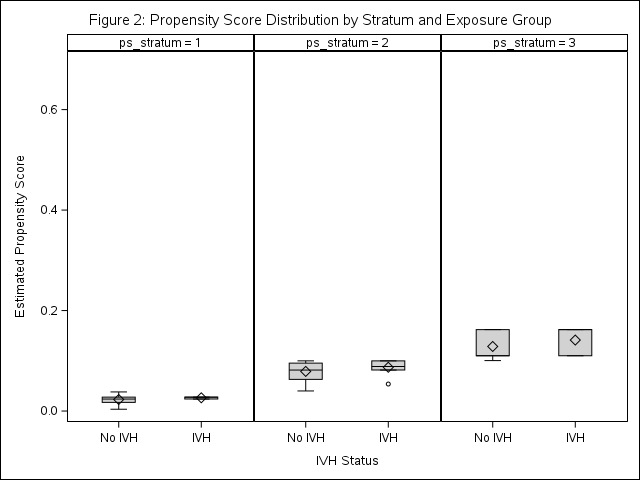
\includegraphics[width=0.48\textwidth,height=\textheight]{fig_ps_distribution_strata_a.png}
&
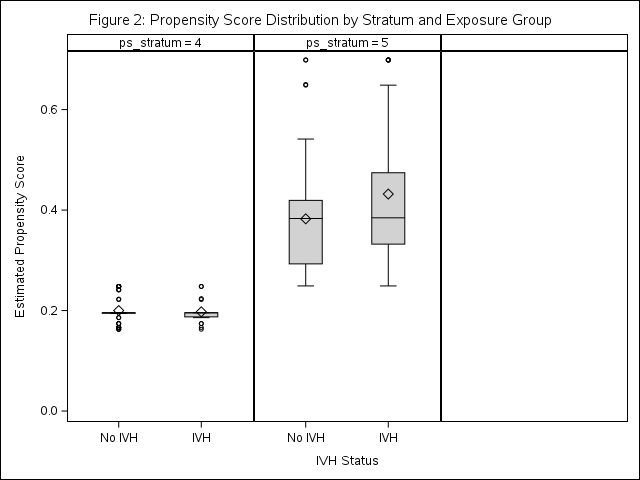
\includegraphics[width=0.48\textwidth,height=\textheight]{fig_ps_distribution_strata_b.png} \\
\bottomrule
\end{longtable}

Within each quintile, the PS distributions for the IVH and No-IVH groups
were fairly close by design. This was especially clear in strata 4 and
5, where most exposed infants were located. The lower three strata
contained very few IVH infants, which again shows limited common support
at the low end of the PS distribution.

\textbf{Plain-language interpretation of the figures:} These plots show
that infants with IVH were much more likely to come from the higher-risk
part of the cohort even before the outcome was considered.
Stratification helps by comparing infants within the same risk bands
instead of comparing very different infants across the full sample.

\begin{center}\rule{0.5\linewidth}{0.5pt}\end{center}

\hypertarget{requirement-4-table-2-comprehensive-comparison-of-effect-estimates}{%
\section{Requirement 4: Table 2 --- Comprehensive Comparison of Effect
Estimates}\label{requirement-4-table-2-comprehensive-comparison-of-effect-estimates}}

I compared six approaches for the IVH-mortality association:

\begin{enumerate}
\def\labelenumi{\arabic{enumi}.}
\tightlist
\item
  \textbf{Unadjusted:} simple regression with IVH only.
\item
  \textbf{Adjusted (HW1):} multivariable regression with IVH,
  pneumothorax, birth weight category, and gestational age category.
\item
  \textbf{PS Matched (HW3):} 1:1 matched analysis.
\item
  \textbf{PS IPTW (HW4):} weighted GEE with ATE weights.
\item
  \textbf{PS Stratification (HW5):} conditional logistic regression by
  PS quintile for OR and Poisson regression adjusted for PS stratum for
  RR.
\item
  \textbf{PS Regression (HW5):} regression adjusted for the estimated PS
  and its squared term.
\end{enumerate}

\hypertarget{table-2-effect-estimates-ivh-vs.-no-ivh-on-mortality}{%
\subsection{Table 2: Effect Estimates --- IVH vs.~No IVH on
Mortality}\label{table-2-effect-estimates-ivh-vs.-no-ivh-on-mortality}}

\begin{longtable}[]{@{}
  >{\raggedright\arraybackslash}p{(\columnwidth - 8\tabcolsep) * \real{0.17}}
  >{\centering\arraybackslash}p{(\columnwidth - 8\tabcolsep) * \real{0.21}}
  >{\centering\arraybackslash}p{(\columnwidth - 8\tabcolsep) * \real{0.21}}
  >{\centering\arraybackslash}p{(\columnwidth - 8\tabcolsep) * \real{0.21}}
  >{\centering\arraybackslash}p{(\columnwidth - 8\tabcolsep) * \real{0.21}}@{}}
\toprule
& Dead = 0 & Dead = 1 & ORs (95\% CI) & RRs (95\% CI) \\
\midrule
\endhead
\textbf{IVH} & & & & \\
 No & 372 (86.5\%) & 58 (13.5\%) & Referent & Referent \\
 Yes & 43 (51.2\%) & 41 (48.8\%) & & \\
\textbf{Unadjusted} & & & 6.12 (3.67, 10.18) & 3.62 (2.43, 5.40) \\
\textbf{Adjusted ORs/RRs} & & & & \\
 Multivariable model (HW1 purposeful selection) & & & 4.15 (2.29, 7.52)
& 2.06 (1.35, 3.14) \\
 PS Matched (HW3, 82 pairs) & & & 3.86 (1.68, 8.86) & 2.05 (1.35,
3.12) \\
 PS IPTW ATE (HW4) & & & 3.34 (1.65, 6.76) & 2.45 (1.53, 3.90) \\
 \textbf{PS Stratification (HW5)} & & & \textbf{3.42 (1.97, 5.92)} &
\textbf{2.18 (1.42, 3.35)} \\
 \textbf{PS Regression (HW5)} & & & \textbf{3.38 (1.94, 5.91)} &
\textbf{2.15 (1.38, 3.35)} \\
\bottomrule
\end{longtable}

\emph{Dead = 0/1 counts show row percentages from the original
unweighted cohort (N = 514). In the HW5 PS-stratified analysis, the OR
came from conditional logistic regression with PS stratum as the
stratification factor, and the RR came from Poisson regression adjusted
for PS stratum. In the HW5 PS-regression analysis, the PS and PS-squared
terms were included in the model to allow a non-linear PS-outcome
relationship.}

\textbf{Plain-language interpretation of Table 2:}

\begin{itemize}
\item
  \textbf{Unadjusted (OR = 6.12; RR = 3.62):} In the crude analysis,
  infants with IVH had a much higher risk of death than infants without
  IVH. This estimate was probably too large because the IVH group was
  also much sicker at baseline.
\item
  \textbf{Multivariable-adjusted, HW1 (OR = 4.15; RR = 2.06):} After
  adjusting for pneumothorax, birth weight, and gestational age, the
  effect estimate became smaller. This shows that confounding was
  important, but IVH still remained associated with roughly a two-fold
  higher risk of death.
\item
  \textbf{PS-Matched, HW3 (OR = 3.86; RR = 2.05):} The matched analysis
  gave almost the same RR as the HW1 adjusted model. That is reassuring
  because two different approaches gave nearly the same answer.
\item
  \textbf{PS-IPTW, HW4 (OR = 3.34; RR = 2.45):} The IPTW analysis also
  showed higher mortality in the IVH group. The weighted RR was somewhat
  larger than the HW1 and HW3 estimates, which may reflect the effect of
  large weights and some residual imbalance.
\item
  \textbf{PS Stratification, HW5 (OR = 3.42; RR = 2.18):} After
  comparing infants within PS quintiles, IVH was still associated with
  about \textbf{2.18 times the risk of death}. This means the elevated
  mortality was not explained away by the measured baseline risk factors
  used to create the PS.
\item
  \textbf{PS Regression, HW5 (OR = 3.38; RR = 2.15):} When I adjusted
  directly for the PS in the outcome model, the result was almost
  identical to the stratified analysis and very close to the HW1 and HW3
  estimates.
\item
  \textbf{Preferred measure:} I prefer the \textbf{risk ratio} here
  because death is not a rare outcome in this dataset, especially among
  infants with IVH. Across the adjusted analyses, the RR estimates
  ranged from about \textbf{2.05 to 2.45}, so the overall conclusion is
  highly consistent.
\end{itemize}

Overall, all six methods point in the same direction: IVH is associated
with substantially higher neonatal mortality in VLBW infants. The crude
estimate was the largest. After adjustment, most methods clustered
around a two-fold increase in risk, which suggests that the finding is
robust.

\hypertarget{comments-on-multivariable-regression-and-ps-methods}{%
\subsection{Comments on Multivariable Regression and PS
Methods}\label{comments-on-multivariable-regression-and-ps-methods}}

\begin{itemize}
\tightlist
\item
  \textbf{Multivariable regression:} easy to fit and uses the full
  cohort, but covariate balance is less transparent and the estimate
  depends on correct outcome-model specification.
\item
  \textbf{PS matching:} creates directly comparable groups, but some
  observations are discarded and precision can decrease.
\item
  \textbf{PS IPTW:} preserves the full cohort and targets a
  population-average effect, but can be unstable when extreme weights
  are present.
\item
  \textbf{PS stratification:} is intuitive and easy to explain, but
  residual confounding can remain within each stratum if overlap is
  limited.
\item
  \textbf{PS regression:} is efficient and simple, but still relies on
  correct modeling of the PS term in the outcome model.
\end{itemize}

In this dataset, the HW1 multivariable model, the HW3 PS-matched model,
the HW5 PS-stratified model, and the HW5 PS-regression model all gave
very similar adjusted RRs. That consistency strengthens the evidence
that IVH is independently associated with neonatal mortality and is not
simply a marker of lower birth weight or shorter gestation.

\begin{center}\rule{0.5\linewidth}{0.5pt}\end{center}

\hypertarget{summary}{%
\section{Summary}\label{summary}}

Using the main-effects PS model (C-statistic = 0.771), I created five PS
quintile strata and then estimated the association between IVH and
mortality using PS stratification and PS regression. The final
PS-stratified estimate was \textbf{OR = 3.42 (95\% CI: 1.97, 5.92)} and
\textbf{RR = 2.18 (95\% CI: 1.42, 3.35)}. The final PS-regression
estimate was \textbf{OR = 3.38 (95\% CI: 1.94, 5.91)} and \textbf{RR =
2.15 (95\% CI: 1.38, 3.35)}.

These two HW5 estimates were highly consistent with the adjusted HW1
model and the PS-matched HW3 model, while the IPTW estimate from HW4 was
somewhat larger. My overall conclusion is unchanged: among VLBW infants,
IVH is associated with about a \textbf{two-fold higher risk of death}
after accounting for measured baseline confounding.

\begin{center}\rule{0.5\linewidth}{0.5pt}\end{center}

\hypertarget{appendix}{%
\section{Appendix}\label{appendix}}

The SAS program for this homework is provided as a separate file:
\texttt{HW5\_Analysis.sas}.

\end{document}
